%
% ****
\chapter{Einleitung}
% ****
%

\begin{figure}[!h] %[!t] ...
  \centering
  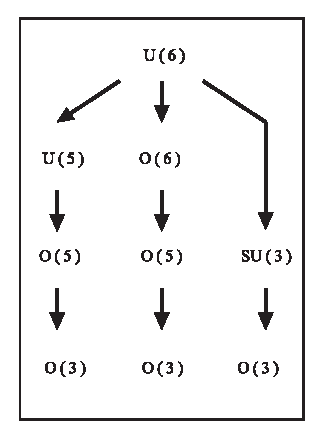
\includegraphics[width=4cm]{figure}
  \caption{Die Bildunterschrift sollte eine sinnvolle Erläuterung der
    Darstellung geben und ist immer mit einem Satzpunkt abzuschließen.}
  \label{fig:abbildung1}
\end{figure}

%%% Local Variables: 
%%% mode: latex
%%% TeX-master: "main"
%%% End: 
